% !TeX root = ../main.tex
% Add the above to each chapter to make compiling the PDF easier in some editors.


\chapter{Case study}\label{chapter:EA documentation in an insurance company} 
% IST-Analyse
% EA documentation in an insurance company

This chapter introduces in the first section the case study. The second section will explain the factors that influence the IT landscape of the insurance company. These are divided into internal and external factors. In the next section~\ref{section:asislandscape} the IT landscape is explained. The current method of the EA documentation process in the insurance company is explained. The EAD process was conducted during this  master-thesis.
In the following section~\ref{section:targetitlandscape} the target IT landscape will be described.
At the end of this chapter in section~\ref{section:derivedrequirements}, the derived requirements to automated the EA relevant information collection process will be presented to introduce the new approach for an automated EAD.

\section{Case Study Design}\label{section:casestudy}

The case study was conducted according to the research methodology for software engineering from Per Runeson. \hl{Per Runeson, 2008}

\subsection{Case study objectives}\label{subsection:casestudyobjectives}

This case will identify the current practice and the challenges regarding the EAD process in a german insurance company. To goal of the case study is to derive requirements for an automated EAD process and compare these with the findings of the literature research to improve to develop an automated process out of the requirements.

\subsection{Case study definition}\label{subsection:casestudyobjectives}

The subject of this case study is a international insurance company based in Munich. The investigation in this case will mainly focus on the Enteprise Architecture Documentation process within the company. To understand the process, the study will take a look at the IT landscape to retrieve information how the EA relevant components interact with each other and what factors influence the IT landscape. This will give an overview to find out why the enterprise is documenting EA relevant information in that way.

\subsection{Case study methodology}\label{subsection:casestudymethodology}

\subsubsection{Research questions -  what to know?}
%How  to  assign  the  application  landscape  to  business  domains?
%How  to  obtain  EA  relevant  information  from  the  runtime  behaviour  ofcloud-based environments?
%How to automate the assignment process with an integrated toolchain?
%How  does  a  prototype  implementation  of  the  automated  documentationprocess of cloud applications look like?
The research questions that are going to be answered are mentioned in ~\ref{section:researchquestions}.
RQ1 and RQ3 are relevant for the case study. The aim is to see if the questions can be answered during the case study to derive requirements to improve the EAD.

\subsubsection{Methods — how to collect data?}

As mentioned by Runeson et al. \hl{Per Runeson, 2008} the following information sources can be used to collect data:

\begin{itemize}
    \item Different data sources
    \item Archival data
    \item Interviews
\end{itemize}

%Archival data refers to, for example, meeting minutes, documents from different development phases, organizational charts, financial records, and previously collected measurements in an organization

During the case study a literature research was conducted to derive challenges and requirements from literature to be able to compare the information to the of current situation the company.

An analysis of the archived data of the company was executed during the thesis in order to gain more knowledge about the IT landscape, the reasons of the current documentation process, projects changing the landscape and its documentation and what the enterprise expects to be improved or even automated.

To retrieve more information informal and semi-structured interviews were conducted.The interviews were divided into 2 parts. The first part explained the motivation and the objectives of the thesis. The motivation introduced a brief overview of the scope of the thesis and the objectives includes the research questions to be answered. The second part of the interview consisted of questions regarding the findings during the research of the current situation.

\section{Factors influencing the IT landscape}\label{section:influencingfactors}

This section will describe the influencing factors that have an impact on the IT landscape of the german insurance company. To understand the IT landscape an overview of the main influencing factors is presented. First, the internal factors are explained. Secondly, the external factors such as regulations will be mentioned. Finally, EA documentation process will be described. 

\subsection{External factors}\label{subsection:externalinfluencingfactors}

The section will describe the most important external factors that change the IT landscape of the enterprise and thus have an impact on the EAD. There are three regulations that mainly influence the EAM. The first regulation is the General Data Protection Regulation (GDPR). The second factor affecting the IT landscape is the VAIT Regulation. The last regulation influencing the IT landscape is the international standard ISO 22301.

\subsubsection{General Data Protection Regulation}

The General Data Protection Regulation (GDPR) is a European Data Protection Regulation that enforces all member states of the European Union to harmonize data privacy laws. The GDPR is related to processing of personal data. It assures fundamental rights of  persons, especially the right to the protection of personal data.

\subsubsection{VAIT Regulation}

The regulation "Versicherungsaufsichtliche Anforderungen an die IT" (engl. "Insurance supervisory requirements for IT") (VAIT) affects the IT of insurance companies with headquarters in Germany. The use of information technology (IT) in companies, including IT services offered by IT service providers, is of central importance to insurance companies and pension funds. The circular letter published in the context of the regulation mentioned contains information on the interpretation of the regulations on business organization in the Insurance Supervision Act  (in german "Versicherungsaufsichtsgesetz") (VAG) insofar as they relate to the technical organizational equipment of the companies. It makes these regulations binding for Federal Financial Supervisory Authority (in german "Bundesanstalt für Finanzdienstleistungsaufsicht") (BaFin), thereby ensuring consistent application to all companies and groups. The circular letter provides a flexible and practical framework, in particular for the management of IT resources, information risk management and information security management. \hl{Rundschreiben VAIT}

The main requirement affecting the EAD is the IT operations requirement. The IT operation must implement the fulfillment of the requirements resulting from the implementation of the business strategy as well as the IT-supported business processes. The components of the IT systems and their relationships to each other should be managed appropriately and the inventory information collected should be updated regularly and on an ad hoc basis. The stock information includes in particular: Inventory and purpose of the components of the IT systems with the relevant configuration information, location of the components of the IT systems, compilation of the relevant information on warranties and other support contracts (possibly linking), information on the expiration date of the support period of the components of the IT systems, accepted Period of unavailability of the IT systems and the maximum tolerable data loss. \hl{Rundschreiben VAIT}

\subsubsection{ISO 22301}

The ISO 22301 standard represents the latest international policy for Business Continuity Management (BCM) and was released in 2012. Its objective is to assist in the reduction of business interruptions due to unforeseen emergencies. This is the norm an update of the standards ISO 31000 and ISO 27001. It is considered a universal standard in the the sense that they apply to companies of all sizes and regardless of the used technologies.

To ensure the reduction of unforeseen emergencies an IT emergency system should be introduced to act as a a holistic management system. That includes monitoring and regular review of the IT landscape. These two aspects enable one of the main components of the standard execution: the Business Impact Analysis. 

The Business Impact Analysis (BIA) is a complex task that includes important corporate resources as a precautionary measure: specialists, executives and corporate management. The analysis includes the collection and identification of processes and functions,
the required resources such as staff, but also hardware resources like IT facilities, buildings, warehouses with their technical equipment. The analysis also include dependencies on IT processes, the definition of the core processes and impacts and recovery times.
\hl{Springer Notfallplan in Kommunikationsnetzen}

\subsection{Internal concerns}\label{subsection:internalinfluencingfactors}

The internal factors presented in the following paragraphs are mainly the drivers that have an impact on the IT landscape of the enterprise.

\subsubsection{Main business system}

The main legacy system of the insurance company has developed over time into a legacy system. Application components were built to connect new systems or application to enable a communication between those. The added layers, components and adapters led to an not transparent and not maintainable legacy system. To improve the transparency of the legacy system the enterprise decomposed the system into modules to gain information about the dependencies to other applications and/or systems.

\subsubsection{Business Continuity Management}

Driven by the ISO standard 22301 the german insurance company of this case study is also obliged to fulfill this regulation through a BCM project. The company is exposed to increasing risks that endanger the continuous and timely provision of its services to the customer. Contributing to this are various developments and trends in society and the economy, such as growing globalization, increasing networking, centralization, automation, outsourcing.
Due to the increasing complexity of business processes and their increasing dependence on information technology and external service providers, events such as fire, flood or the failure of information technology and external service providers or personnel can have a major impact.

The Business Continuity Management (BCM) is a management process with the aim of early identification of serious risks for the enterprise, which endanger the existence, and to establish measures against them. In order to ensure the viability and thus the existence of the company, appropriate preventive measures must be taken, which on the one hand increase the robustness and reliability of the business processes and on the other hand enable rapid and targeted response in an emergency or crisis.

The goal of the BCM is to ensure that important business processes are not or only temporarily interrupted, even in critical situations, and that the economic existence of the enterprise remains secured even in the event of a major loss event (crisis cases require separate consideration). A holistic view is therefore crucial. Consider all aspects that are required to continue critical business processes when a claim event occurs, not just the Information Technology resource. IT emergency management is part of the BCM.
Critical business processes in the sense of emergency management means "time-critical", so that this process requires a faster resumption of activity, otherwise a high level of damage can be expected. The high damage can result from financial losses, violations of laws or contracts, from image damage or other damage scenarios.
A business process classified as "uncritical" does not mean that it is unimportant to the enterprise, but merely that it has a lower priority in recovery.

\subsubsection{Decommissioning project}

The goal of the decommissioning project is to withdraw traditional data centers from active service to mainly to reduce costs. The decommission of applications or systems can be executed have different reasons. The first reason is to decommission systems due to lack of support available or the purpose to remove old legacy systems. The data of the removed system has to be migrated to the new system. The another reason for decommissioning systems is to withdraw traditional data centers from active service. The efficient redistribution of IT resources can lead to migrations of systems from one data center to another to reduce the amount of running data centers and consequently reduce the costs of running data centers. The other approach of migrating applications to withdraw servers is the migration to the cloud. The elasticity of the cloud enables the efficient use of computational efficiently and has as a consequence that traditional server can be withdrawn.

\subsubsection{Cloud migration project}
%TODO: include sources for this subsection: Chen 2015,  Odun-Ayo 2018
The migration to the cloud of the IT infrastructure is a central and strategic issue. The expansion of the IT architecture, including cloud solutions, forms the basis for digitization and increases the productivity and efficiency of IT processes. The migration improves the availability and scalability of IT services, thereby increasing the growth potential of all IT structures. The duration of the total migration amounts to an estimated 4 years and is divided into quarterly projects. The migrated applications / Minimum Viable Products (MVP) are put into production at the end of the quarter and put into line.

The arguments for migrating to the cloud are divided into two aspects. The arguments covering the first aspect of operations are:
\begin{itemize}
    \item Performance and Availability: OpenShift and CloudFoundry are proven solutions that are used in many large organizations and designed for high availability.
    \item Scalability: OpenShift and CloudFoundry enables fast and easily scalable automation of applications based on demand and load.
    \item Cost Efficiency: Moving from traditional virtualization technology to container technology will bring better utilization of existing resources and, in the long run, cost savings.
    \item Security: OpenShift and CloudFoundry provide easy deployment of security patches for platform and applications. The updates can be imported without downtime for the end user. Both providers also offer easy deployment of security patches for platform and applications. The updates can be imported without downtime for the end user.
\end{itemize}
The following migration arguments cover the second aspect of application development:
\begin{itemize}
    \item Developer Satisfaction: Developers can leverage cutting edge technologies to build innovative solutions.
    \item Developer Efficiency: CloudFoundry is designed as a self-service platform. Developers get more freedom in a well-defined framework to get to their destination faster.
\end{itemize}

The project objectives are:
\begin{itemize}
    \item Full application migration without interruption to ongoing operations (24x7 applications, sales, support and night jobs). These means the technical migration of more than 400 applications.
    \item Create a migration blue print and best practices for dealing with the new infrastructure.
    \item Creation of the migration framework including half / tools to carry out the migration
    \item Supplementing the operational concept for post-migration operations. This means the monitoring and error analysis of the migrated applications after the production has been set for the duration of the project.
\end{itemize}

The project does not include the migration of fat clients and \hl{non-insurance-owned} applications.

\section{AS-IS IT landscape}\label{section:asislandscape}

This section will described the IT landscape of the company. The following picture shows the main components of the IT landscape.

\begin{figure}[htpb]
  \centering
  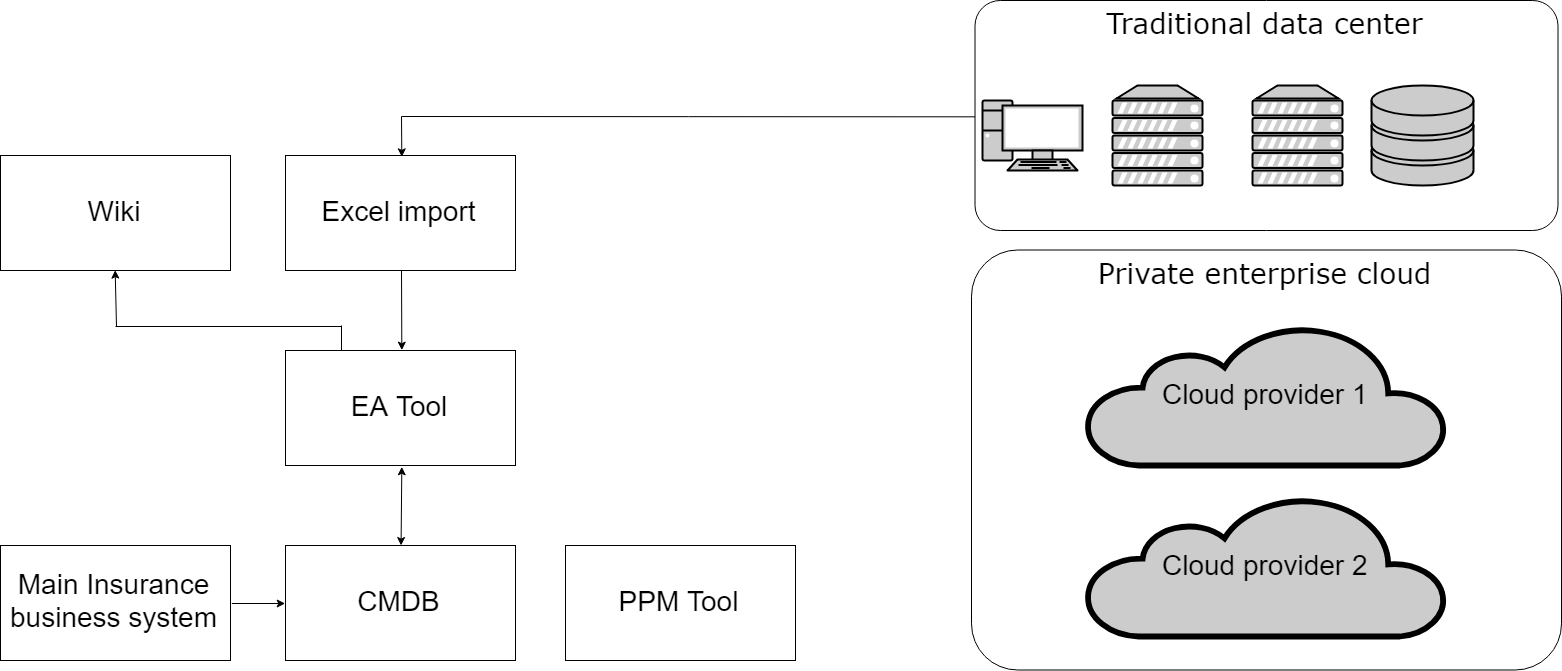
\includegraphics[width=0.8\textwidth]{figures/as-is-it-landscape.png}
  \caption{ AS-IS IT landscape~\parencite{Corpancho Villasana 2018}}
  \label{fig:AS-IS IT landscape}
\end{figure}

The company consists of two environments: the traditional environment which contains traditional data center hardware and its private cloud infrastructure which is divided into two different cloud service providers. The first cloud infrastructure service provider is OpenShift and the second provider is Pivotal's CloudFoundry.

The traditional data centers host the legacy systems of the company and all other kind of applications.

OpenShift is a container platform. The PaaS provider OpenShift offers the possibility to deploy docker containers to its platform and enables the orchestration by Kubernetes. \hl{OpenShift}

CloudFoundry (CF) is an open source, multi-cloud application platform as a service. Similar to Openshift, CF has a container-based architecture which also enables the deployment of applications written in any programming language.

The main components of the IT landscape in regard to EAm are the EA tool, the CMDB, the PPM tool, a service-oriented architecture (SOA) repository, the Wiki s a collaboration software program and the main business system. As shown in the picture above the enterprise uses Iteraplan as their EA tool. %AMUR?
The SOA repository is used for managing services such as WSDLs and XML schema definitions, access rights, information related to the service level agreements and transactional operations of the services. \hl{Enterprise SOA Buch} 
%Enterprise SOA: Service-oriented Architecture Best Practices By Dirk Krafzig, Karl Banke, Dirk Slama
Relevant for the EAM are the other repositories depicted in the picture. Other repositories include change management tools, license management tools, etc.

\subsection{Current EA documentation}\label{subsection:currentead}

The EAD integrates several tools as shown in figure \hl{XXX}. 

\subsubsection{Excel import}

The first EA documentation process was driven by the external mentioned ISO 22301 standard. The enterprise decided to collect the information about the IT landscape. The usage of Microsoft Excel sheets for keeping data is still important for enterprises since many organizations still rely on them for information storing.\hl{}

Initially the systems or applications that are critical for the business were documented. This was mainly driven by the BCM project and the BIA of IT failures. Ensuring that important business process are not interrupted and have no economic impact to the company is essential that the enterprise remains secure. For this initiative a team was created to retrieve this information. The documentation process was done fully manually. Therefore the document containing the information was inconsistent and contained redundant information.

The continuation of the project is mainly driven by the VAIT regulation since enterprise will have to have a fully application inventory.

\subsubsection{Integration of the CMDB}
% Pasarlo a current EA docu?
Due to the BCM regulation mentioned in section~\ref{section:internalinfluencingfactors}, an integration between the EA tool and the CMDB was implemented. The EA tool integrates data from the CMDB. The application developed for the integration retrieved data from the CMDB and imports the data to the EA tool in regular intervals. The import is was unidirectional. Only Business Services were imported from the CMDB. No infrastructure data was integrated into the EA tool. The import did not analyze the data, meaning that if the imported data was redundant there was no merge conflict solved. The integration was developed to improve these challenges. The Integration on the CMDB contains now a conflict solution and harmonizes the redundant imported applications with a unique identifier. The import mechanism also differentiates between a flag set in the CMDB metamodel to import the business services as an application or a technical components. This differentiation is done because in the CMDB everything was modeled as a business service.

This integration was the pilot integration project for information sources to the existing EA tool. Further integrations of different information sources will be implemented due to the successful development of this integration.

The main business system of the enterpise was initially documented in the CMDB. For that reason the information about the main business system was retrieved via the CMDB to the EA tool.

%Semi automated?
The integration of the CMDB to the EA tool is semi-automated since the information of the CMDB was also retrieved manually.

\subsubsection{Export to Wiki}

The export of the collected data in the EA tool was mainly driven by the integration of the CMDB. The goal of the data export to the Wiki was to analyze and evaluate the data of the EA tool. 

Enterprise Wikis enhances sharing and collaboration of employees knowledge. The employees can easily edit the wikis content and provide their knowledge to the information center. The unstructured information can contain file attachments, multimedia content and allows the interlinkage of wiki pages. Referencing EA relevant information such as documents is supported by wikis. To link this references wikis are more appropriate than an EA tool.\hl{Fiedler 2013}

To enable the collaboration and knowledge sharing of the employees knowledge a Wiki was integrated into the IT landscape. A wiki page is created for each application of the EA tool. This enables to collect more data than the metamodel of the EA tool allows. The wiki page contains several characteristics of an application. Some of the extended characteristics of an application are architectural decision, users, architectural diagrams, decommissioning information driven by the decommission concern, operational manual and other notes regarding the application.

\subsubsection{Cloud integration}

As we can see in picture \hl{XXX} there is no integration of the applications running on the cloud-based environments. There is no defined process of the EAD of applications deployed to the cloud.

\section{Target IT Landscape}\label{section:targetitlandscape}

This section will explain the target IT landscape of the company. The target IT landscape is mainly driven by the concerns. The following picture shows the target IT landscape.

\begin{figure}[htpb]
  \centering
  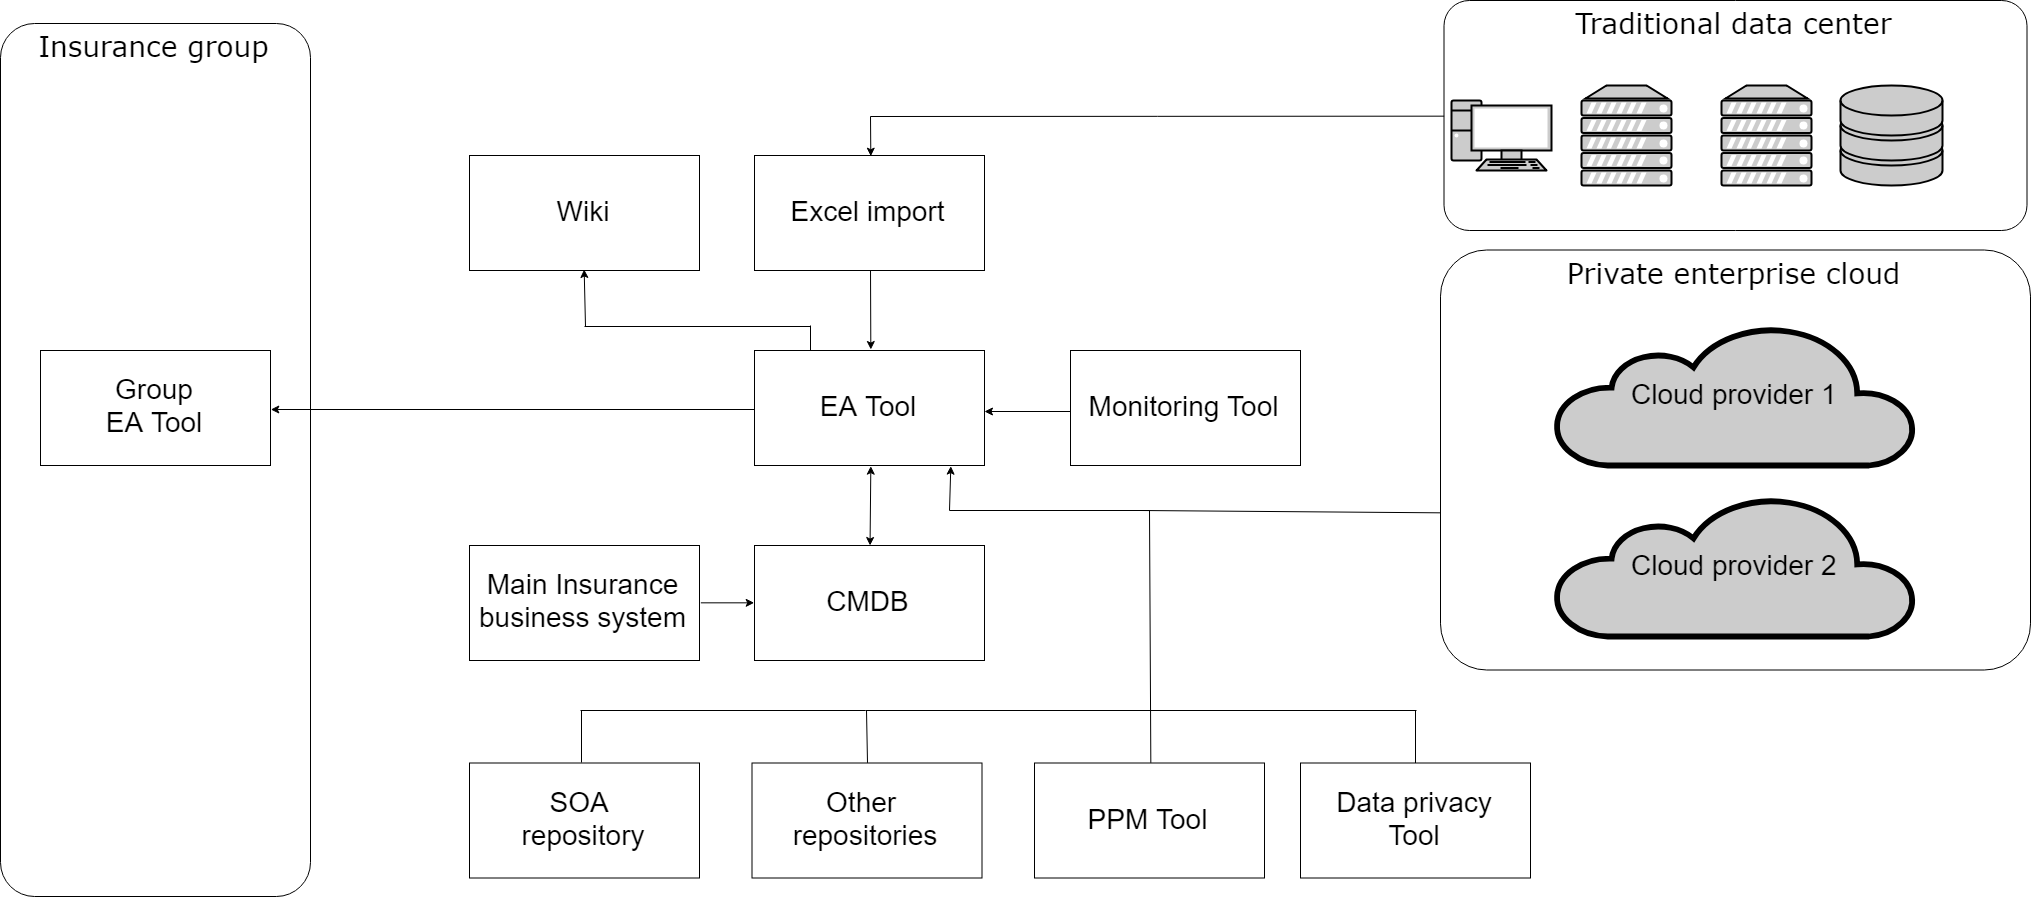
\includegraphics[width=0.8\textwidth]{figures/target-it-landscape.png}
  \caption{ Target IT landscape~\parencite{Corpancho Villasana 2018}}
  \label{fig:Target IT landscape}
\end{figure}

\subsubsection{Integration of data privacy tool}
%Amur für datenschutz
Driven by the GDPR the enterprise has developed a tool which contains a list of applications that are related to this regulation. Therefore an integration of this tool is planned in order to have this specific information in the EA tool.

\subsubsection{Integration of service-oriented architecture repositories}

An integration of a service-oriented architecture (SOA) repository enables the enterprise to include inventories of the web services in a SOA repository to the EA tool. Therefore an integration is intended.

\subsubsection{Integration of other repositories}
The enterprise goal of the enterprise is to interlink different tools containing different EA relevant information. This goal enables a federated architecture to allow information sharing between different data sources. Therefore it will also integrate other repositories such as license management tools and change management tools.

\subsubsection{Integration of the PPM tool}
The main goal of the integration of a PPM Tool is to enable a mapping between the projects and the applications or systems in the enterprise. The EA tool in place contains in its metamodel the entity "project". This allows an integration of the PPM tool to the existing EA tool. The projects of the PPM tool are imported into the EA tools as the entity "project". A manual mapping between the projects and applications is then still required. This EAD process of projects can be seen as semi-automated.

\subsubsection{Integration to the group EA tool}

The insurance company is divided into several subsidiaries around the world.The VAIT regulation is applied to every german insurance company. The german insurance company has its headquarters in Germany so the regulation implies an IT inventory for every subsidiary of the insurance company. Therefore every operating entity (subsidiary) has to export the EA information to the Group entity.

\subsubsection{Cloud integration}

As shown in picture \hl{XXX} the applications running on the cloud-based environments will be integrated to the EA tool. The main driver for this integration is the VAIT regulation. As mentioned in the regulation, an insurance company has to be able to deliver an application inventory of the IT landscape. That includes also applications running on private enterprise clouds. 

In the context of the cloud migration project a new defined process for the deployment of the new developed applications was introduced. The major goal of this defined process is to establish a standardized process for agile teams. The process is divided into a build process and a deployment process.

\begin{figure}[htpb]
  \centering
  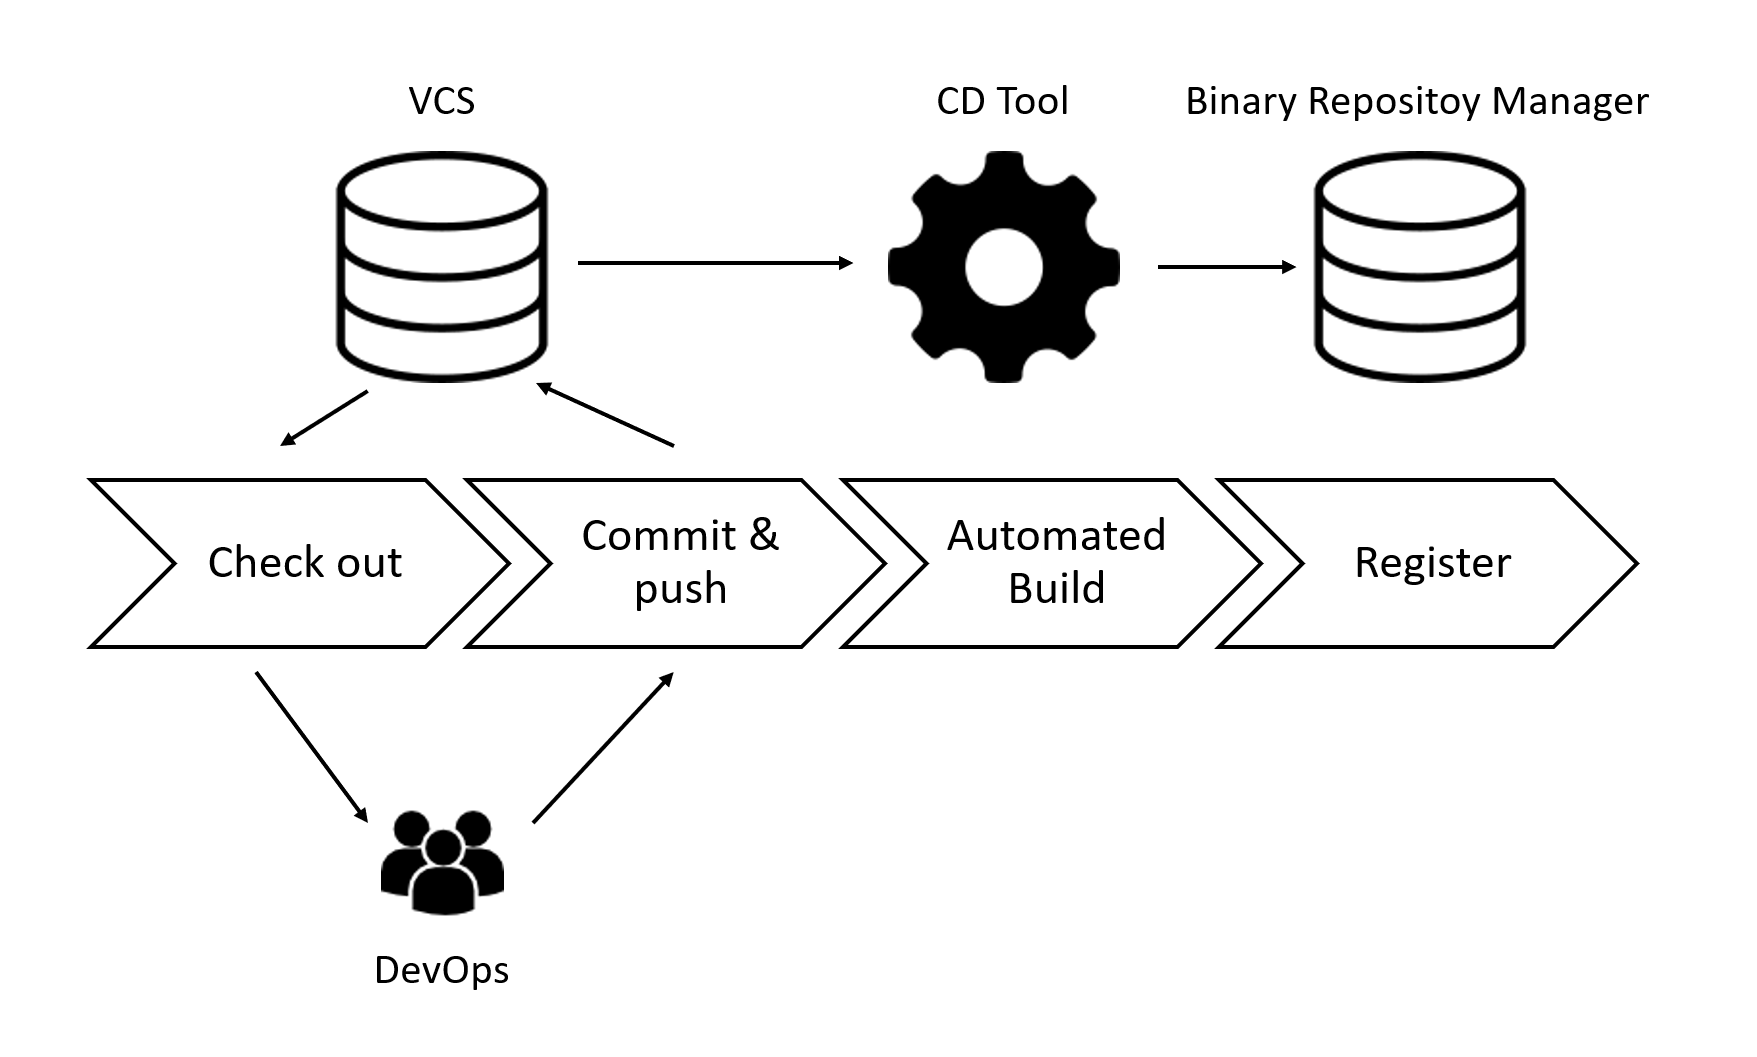
\includegraphics[width=0.8\textwidth]{figures/build-process.PNG}
  \caption{ Build process~\parencite{Corpancho Villasana 2018}}
  \label{fig:Build-process}
\end{figure}

The build process is shown in picture \hl{XXX}. The DevOps team first checks out the latest state of the code from the version control service (VCS). After developing the team commits and pushes the new state back to the VCS repository. The CD tool is constantly monitoring the repository to track changes in the code. If new changes are tracked, the CD tool automatically builds an artifact of the repository and registers the artifact into the binary repository manager tool. That means the built artifact is hosted in the tools and can be downloaded from it.

\begin{figure}[htpb]
  \centering
  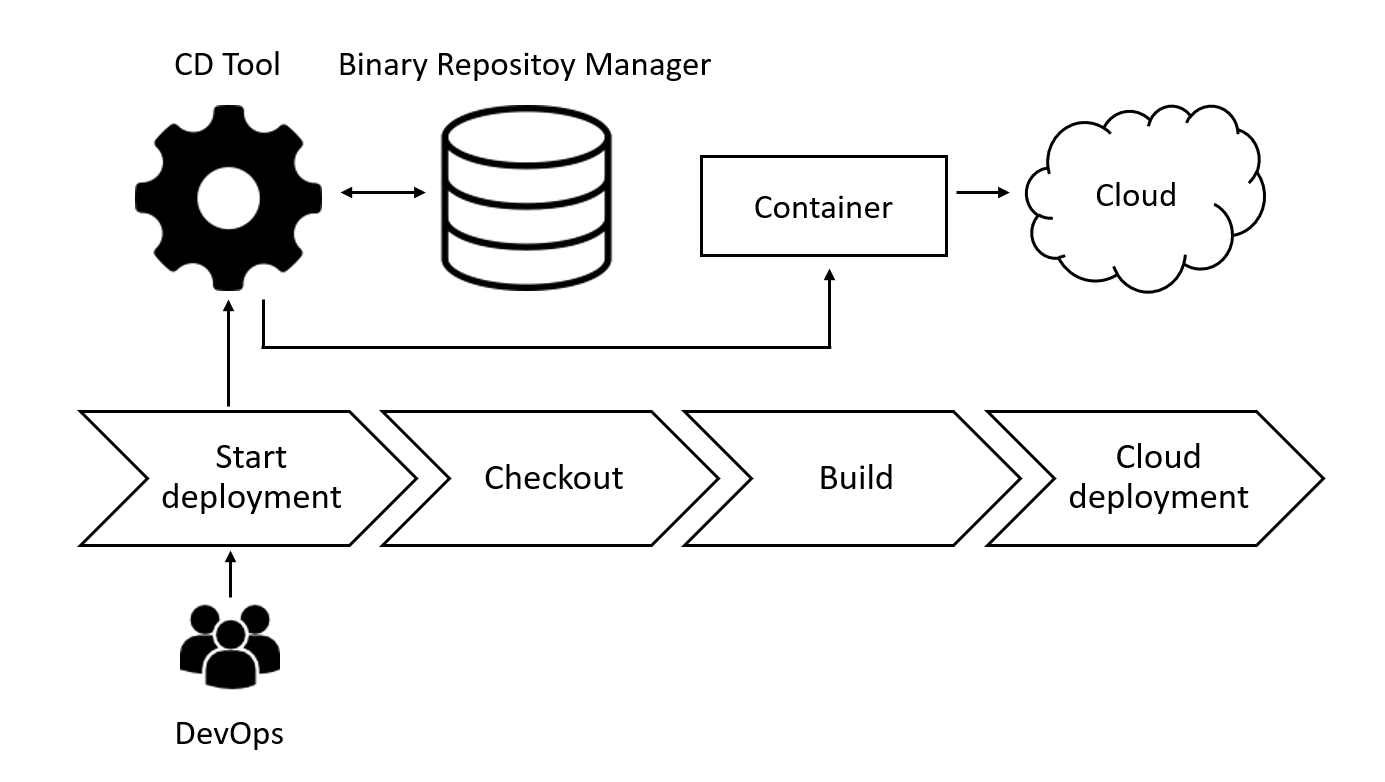
\includegraphics[width=0.8\textwidth]{figures/deployment-process.PNG}
  \caption{ Deployment process~\parencite{Corpancho Villasana 2018}}
  \label{fig:Deployment-process}
\end{figure}

The second part of the defined process is the deployment process as shown in picture \hl{XXX}. The DevOps team triggers manually the deployment process within the CD tool. The tool downloads the latest pushed artifact of the binary repository manager. After downloading the artifact, it build automatically a container out of the artifact. The CD tool pushed then the container to the cloud.

The first approach for a documentation process of the applications running on a cloud-based environment is the establishment of a defined process and a toolchain for building and deploying to the cloud infrastructure. Every application is tracked in the binary repository manager but there is still no integration of the cloud application inventory to the EA tool.

\subsubsection{Monitoring tool integration}

The introduction of a monitoring tool is planned. The reason for establishing a monitoring tool is to gain advantage over the competitors. Monitoring applications allow to retrieve extra information such as individual requests and transactions, resource consumption, reporting and alerting, etc.

The business benefits of monitoring tools for the enterprise are many. One of the benefits is that the enterprise can react quicker to an application failure reducing the revenue loss due to the breakdown of the respective applications or systems. Knowing the failures and obtaining the dependencies from the monitoring tool the enterprise can derive what other systems will be affected by the breakdown. This matches the requirements from the BCM project.

\section{Derived requirements}\label{section:derivedrequirements}

In the previous sections the as-is and target landscape of an insurance company were presented. These sections cover various aspects of the EAD within the studied company. The case study shows different outlooks for future integrations. From the introduced case study, requirements can be derived for for an automated EAD. The following table presents the derived requirements:

\begin{table}[htpb]
  \caption[Automated EAD requirements derived from the case study]{Automated EAD requirements derived the case study}\label{tab:sample}
  \centering
  \begin{tabular}{l l l}
    \toprule
      Id & Requirement\\
    \midrule
      RC1 & Business Impact Analysis of applications\\
      RC2 & Data privacy compliance\\
      RC3 & Integration of a PPM tool\\
      RC4 & Integration of other repositories\\
      RC5 & Integration of cloud infrastructure\\
      RC6 & Integration of a monitoring tool\\
    \bottomrule
  \end{tabular}
\end{table}

\textbf{RC1}: A Business Impact Analysis of applications is not only required by the enterprise, it is also required due to regulations. The enterprise can analyze in case of a sinister what applications are affected and which related systems are implied by a failure. It can quantify the economic impact of failures.

\textbf{RC2}: Tools have to be compliant with the data privacy regulation. An enterprise needs to know what applications store personal data. 

\textbf{RC3}: The integration of a PPM tool is desired by the enterprise to relate projects to applications.

\textbf{RC4}: An integration of other repositories is required by the enterprise to relate information and propagate information sharing.

\textbf{RC5}: The integration of cloud infrastructure is needed due to a full application inventory required by law and due to strategic decisions as migrating to cloud infrastructure.

\textbf{RC6}: An integration of a monitoring tool is planned at the enterprise to increase the reaction time between the failure of a system and the enterprise. Thus, the monetary impact can reduced.
%BIA
%Migration derivations
%cloud documentation process definition: define process how to document apps.
% automated integration

%top down architecture greefhorst und proper
%architetkruprinzipien meistens auf confluence, copas



%bei architekturüberprüfung gesamt architektur (12factorapp) für konzept oder prototyp

%sozialen druck, transparenz für 12 factors, belt
%aier2018: regeln, steuerung und gehorsam oder "einfach mal laufen lassen
%nudging? - shun long hong
%








